\documentclass[12pt]{ctexart}
\usepackage{amsmath} % 用于数学公式
\usepackage{graphicx} % 用于插入图片

\usepackage{minted}
\usepackage{xcolor}

% 设置代码高亮风格
\usemintedstyle{friendly} % 推荐 vs, borland, 或 friendly

% 全局设置
\setminted{
    linenos,            % 显示行号
    breaklines,         % 自动换行
    frame=lines,        % 上下边框
    framesep=2mm,       % 边框间距
    fontsize=\footnotesize, % 字体小一号，适合放入附录
    baselinestretch=1.0,    % 行间距
    tabsize=4
}

% 专门针对 Matlab 的设置 (可选)
\setminted[matlab]{
    mathescape,         % 允许在注释里写公式
}

\usepackage{float}    % 用于控制图表浮动位置

\usepackage{booktabs} % 用于创建更美观的三线表
\usepackage{siunitx}  % 用于标准地排版物理单位和数值
\usepackage{amsmath}  % 用于数学公式环境
\sisetup{per-mode=symbol} % 设置单位格式，例如 m/s

\usepackage{fancyhdr}   % 用于自定义页眉页脚
\usepackage{caption}   % 用于自定义图表标题
\usepackage{subcaption} % 用于子图环境
\usepackage[colorlinks, linkcolor=black]{hyperref}  % 用于创建超链接
\usepackage{makecell}
\usepackage{multirow}  

% \pdfcompresslevel=9

\graphicspath{{./figures/}}

\usepackage[left=2.5cm, right=2.5cm, top=2cm, bottom=2cm]{geometry}

\setlength{\jot}{6pt} % 增加多行公式之间的行距

\linespread{1.5}

\pagestyle{fancy}
% \fancyhead[C]{信号与系统实验大作业}

\begin{document}

% \maketitle
\thispagestyle{empty}

\begin{figure}[t]
    \centering
    
\includegraphics[width=13cm]{./figures/logo1.png}
\end{figure}

\vspace*{\fill}
    \begin{center}
        \Huge\textbf{信号与系统实验大作业报告}
    \end{center}
\vspace*{\fill}

\begin{table}[H]
    \centering
    \large
    \begin{tabular}{ll}
    \textbf{课程:} & 信号与系统实验 \\
    \textbf{姓名:} & 郭浩然 \\
    \textbf{学号:} & 2024303980 \\
    \textbf{桌号:} & 18 \\
    \textbf{班级:} & 10班 \\
    \textbf{学院:} & 民航学院 \\
    \textbf{专业:} & 飞行器控制与信息工程 \\
    \textbf{时间:} & \today \\
    \end{tabular}
\end{table}

\newpage

\tableofcontents
\newpage

% 接在你的 \tableofcontents \newpage 之后

% =========================================================
% 正文开始
% =========================================================

\section{实验概述与设计目标}

\subsection{实验背景}
语音信号处理是数字信号处理领域的重要应用方向。在实际通信与音频处理中，信号常受环境噪声干扰，或需根据场景对语音进行变调、变速处理。本次实验旨在运用《信号与系统》课程中的采样定理、离散时间傅里叶变换（DTFT）、Z变换及数字滤波器设计原理，解决具体的音频处理问题。

\subsection{实验任务要求}
本次大作业包含四个主要任务，涵盖从噪声抑制到语音特效处理的过程：
\begin{enumerate}
    \item \textbf{特定频率噪声抑制}：针对叠加了 \SI{1800}{\hertz} 单频正弦噪声的语音信号，设计数字滤波器进行滤除，尽可能保留原语音频谱特征。
    \item \textbf{变调不变速处理}：基于短时傅里叶变换（STFT）或相关算法，实现男声与女声转换，要求音调改变但语速不变。
    \item \textbf{变速不变调处理}：实现语音的快放与慢放，要求语速改变但音调（基频）不变。
    \item \textbf{语音倒放处理}：实现音频的时域翻转，并分析其时频特性。
\end{enumerate}

本报告将阐述上述任务的原理、算法设计、实现步骤及结果分析。

\newpage

% =========================================================
% 任务一：特定频率噪声抑制
% =========================================================

\section{任务一：特定频率噪声抑制系统设计}

\subsection{问题分析}
本任务需去除叠加在语音信号上的 \SI{1800}{\hertz} 正弦噪声 $n(t) = \sin(2\pi \cdot 1800 t)$。
人声频率范围通常在 \SI{300}{\hertz} 至 \SI{3400}{\hertz}，\SI{1800}{\hertz} 位于人声能量集中的频段。若采用普通带阻滤波器，会切除较多有效频率成分，导致语音清晰度下降或音色沉闷。

因此，需要设计一个具有极窄阻带的带阻滤波器（陷波器）。该滤波器仅对 \SI{1800}{\hertz} 附近的频率产生较大衰减，对其他频率保持单位增益。

\subsection{基于零极点配置法的陷波器设计原理}
为了获得较好的陷波效果，采用基于Z平面零极点配置的方法设计陷波器。

\subsubsection{数字频率的确定}
设采样频率为 $F_s$（实验中由 audioread 获取），噪声频率 $f_0 = \SI{1800}{\hertz}$。则需滤除的数字角频率 $\omega_0$ 为：
\begin{equation}
    \omega_0 = 2\pi \frac{f_0}{F_s}
\end{equation}

\subsubsection{带宽控制的几何解释}
利用 Z 平面的几何矢量法配置零极点。系统的幅频响应 $|H(e^{j\omega})|$ 取决于单位圆上的频率点 $e^{j\omega}$ 到零点距离之积与到极点距离之积的比值：
\begin{equation}
    |H(e^{j\omega})| \propto \frac{\prod |e^{j\omega} - z_k|}{\prod |e^{j\omega} - p_k|}
\end{equation}

当 $\omega = \omega_0$ 时，采样点与零点 $z_1$ 重合，增益为 0，实现陷波。
当频率稍有偏离 ($\omega = \omega_0 + \Delta\omega$) 时：
\begin{itemize}
    \item 若仅有零点，阻带会较宽。
    \item 引入极点 $p_1$ 后，由于 $p_1$ 与 $z_1$ 非常接近 ($r \approx 1$)，采样点到极点的距离也会迅速增加。分母增加抵消了分子增加，使增益迅速回升至 1 (\SI{0}{\decibel})。
\end{itemize}
因此，极径 $r$ 越接近 1，过渡带越陡峭，频率选择性越好。

\subsubsection{零点与极点的配置}
滤波器系统函数 $H(z)$ 由零极点决定。
\begin{itemize}
    \item \textbf{零点设计}：为消除频率 $\omega_0$，在 Z 平面单位圆角度 $\pm \omega_0$ 处设置共轭零点 $z_1, z_2$。
    \begin{equation}
        z_1 = e^{j\omega_0}, \quad z_2 = e^{-j\omega_0}
    \end{equation}
    
    \item \textbf{极点设计}：为防止阻带过宽，在零点附近放置共轭极点 $p_1, p_2$。极点位于单位圆内以保证稳定，且极径 $r$ 取接近 1 的值（本实验取 $r = 0.99$），以获得窄带宽。
    \begin{equation}
        p_1 = r e^{j\omega_0}, \quad p_2 = r e^{-j\omega_0} \quad (0 < r < 1)
    \end{equation}
\end{itemize}

\begin{figure}[H]
    \centering
    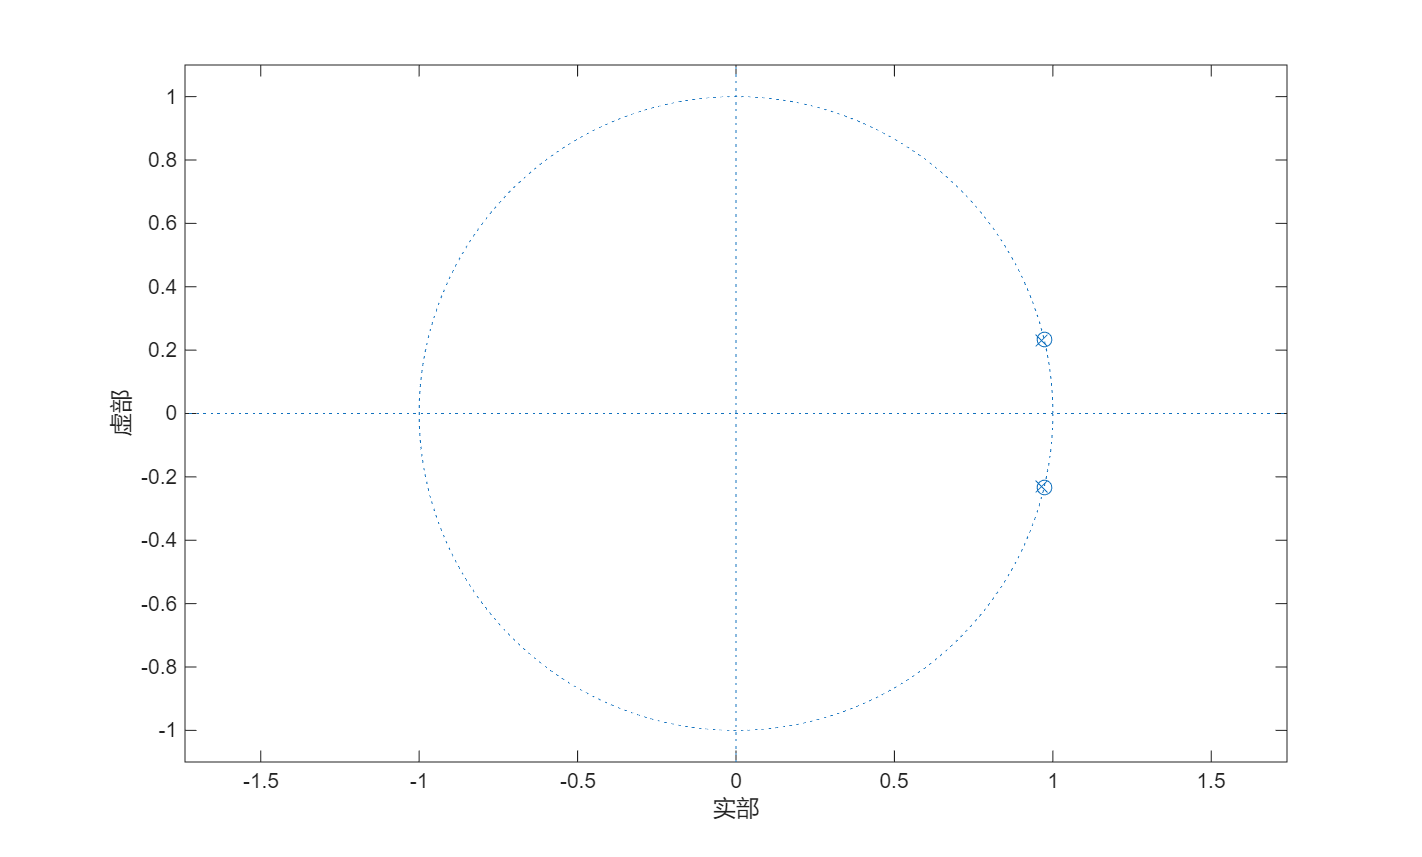
\includegraphics[width=0.9\textwidth]{./task1/zplane.png} 
    % \fbox{\parbox[c][8cm][c]{10cm}{\centering [此处插入MATLAB生成的零极点分布图 (zplane)] \\ 展示单位圆上的零点和极点位置}}
    \caption{设计的1800Hz陷波器零极点分布示意图}
    \label{fig:pole_zero}
\end{figure}

\subsection{系统函数推导}
二阶陷波器的系统传递函数 $H(z)$ 表示为：
\begin{equation}
    H(z) = b_0 \frac{(z - z_1)(z - z_2)}{(z - p_1)(z - p_2)}
\end{equation}
其中 $b_0$ 为归一化增益系数，选取使得直流分量（$\omega=0$）处增益为1。

展开得：
\begin{align}
    \text{分子} &= z^2 - (z_1 + z_2)z + z_1 z_2 = z^2 - 2\cos(\omega_0)z + 1 \\
    \text{分母} &= z^2 - (p_1 + p_2)z + p_1 p_2 = z^2 - 2r\cos(\omega_0)z + r^2
\end{align}

系统函数 $H(z)$ 标准形式为：
\begin{equation}
    H(z) = b_0 \frac{1 - 2\cos(\omega_0)z^{-1} + z^{-2}}{1 - 2r\cos(\omega_0)z^{-1} + r^2 z^{-2}}
\end{equation}

\subsection{幅度频率响应分析}
分析幅频响应 $|H(e^{j\omega})|$：当 $\omega = \omega_0$ 时增益极小；当 $\omega$ 远离 $\omega_0$ 时，增益趋近于 1。

\begin{figure}[H]
    \centering
    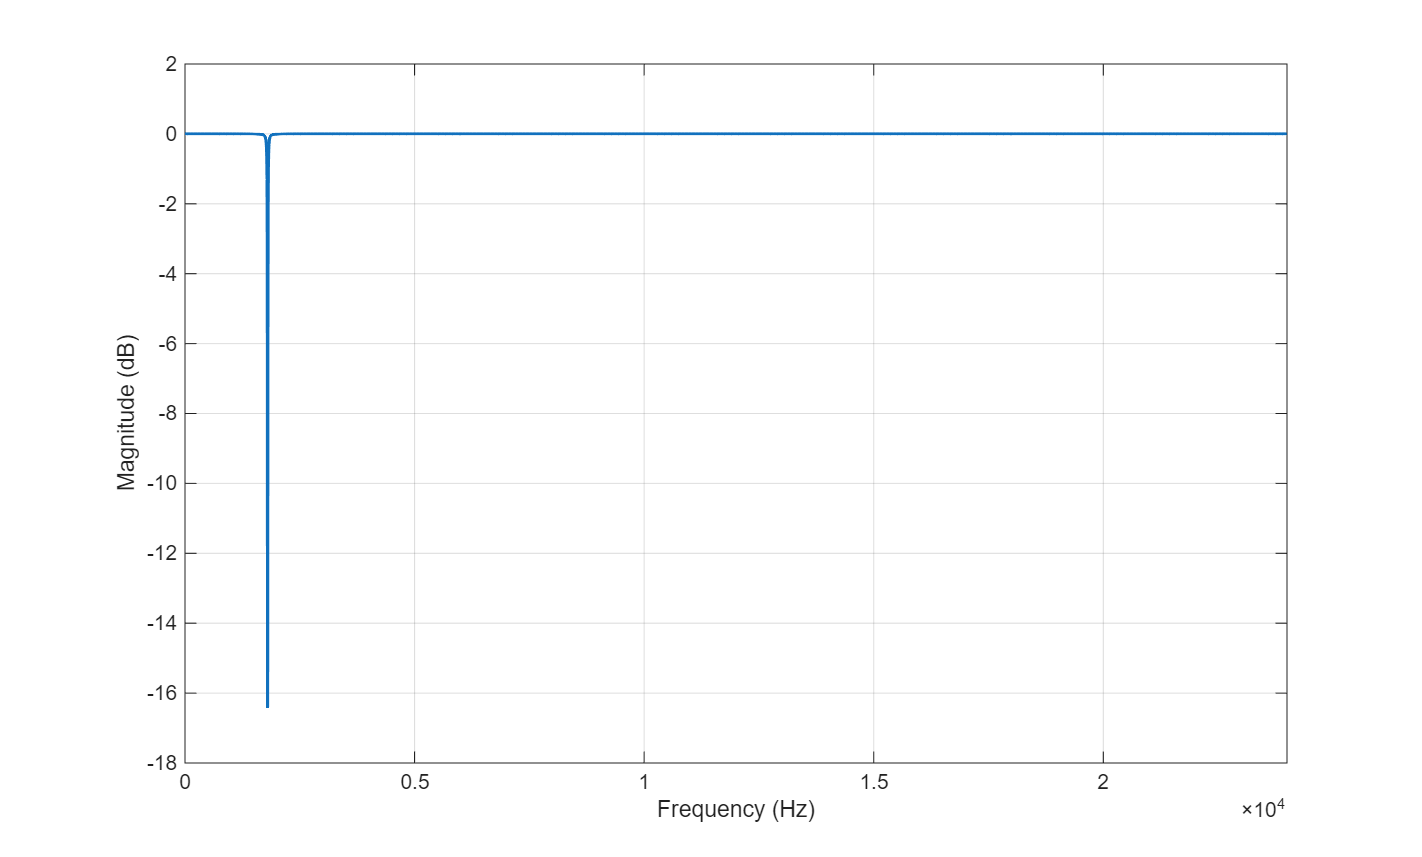
\includegraphics[width=0.7\textwidth]{./task1/freqz.png}
    % \fbox{\parbox[c][8cm][c]{12cm}{\centering [此处插入MATLAB生成的幅频响应和相频响应图 (freqz)] \\ 重点展示1800Hz处的深坑}}
    \caption{设计的陷波器幅频响应特性曲线}
    \label{fig:freq_response}
\end{figure}

\subsection{实验结果与分析}

对信号进行FFT分析，处理前后频谱如图 \ref{fig:task1_spectrum} 所示。
\begin{itemize}
    \item \textbf{加噪信号}：在 \SI{1800}{\hertz} 处存在明显尖峰。
    \item \textbf{滤波信号}：\SI{1800}{\hertz} 处尖峰消失，周围语音频谱成分（\SI{1000}{\hertz} 至 \SI{3000}{\hertz}）保留较好。
\end{itemize}
结果表明该陷波器能有效抑制单频噪声。

\begin{figure}[H]
    \centering
    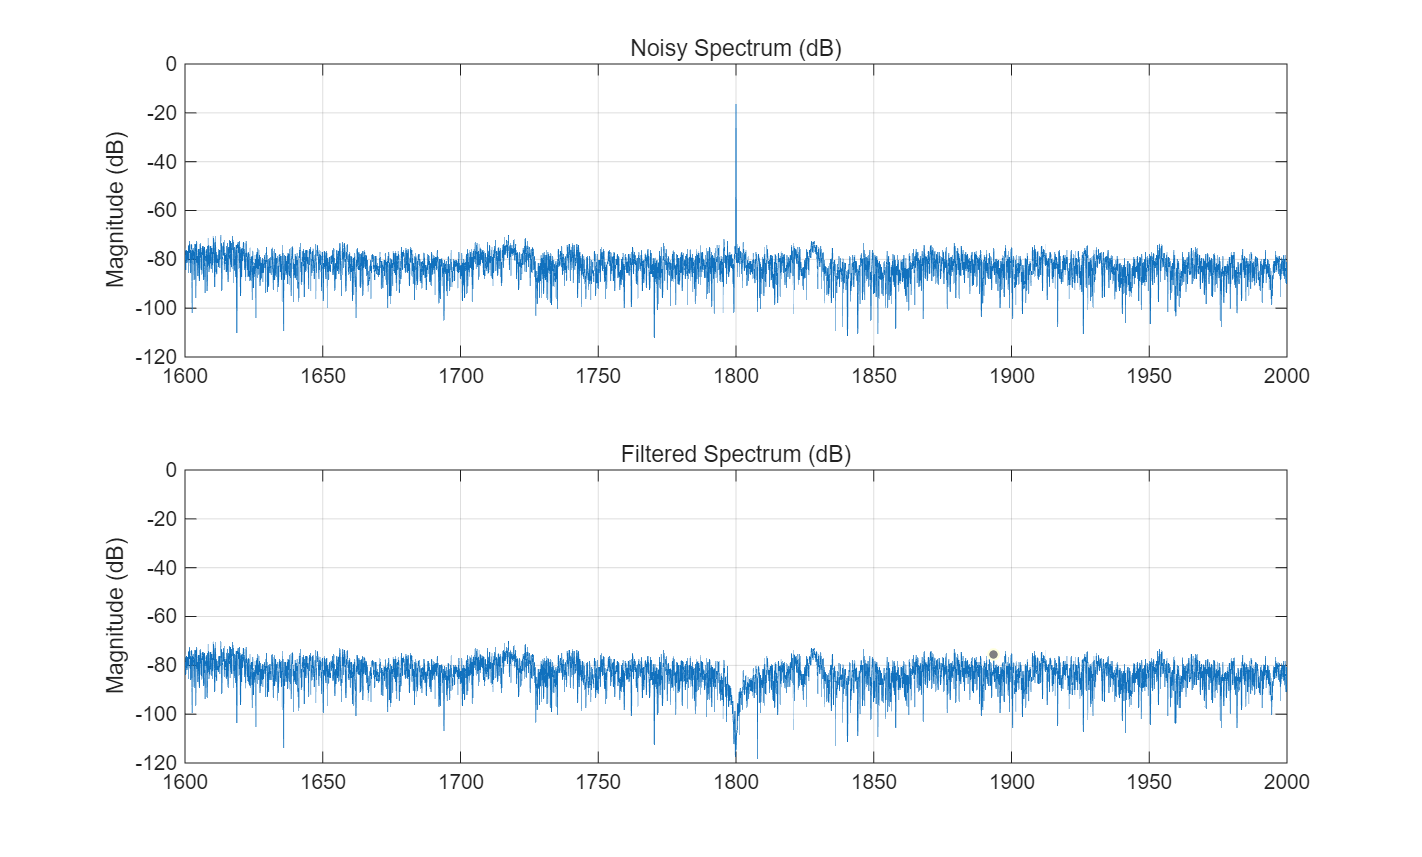
\includegraphics[width=\textwidth]{./task1/spectrum.png}
    % \fbox{\parbox[c][10cm][c]{14cm}{\centering [此处插入频谱对比图] \\ 必须清晰展示1800Hz处的尖峰及其消除情况}}
    \caption{噪声抑制前后的频谱对比分析}
    \label{fig:task1_spectrum}
\end{figure}

\newpage

% % =========================================================
% % 任务四：语音倒放处理
% % =========================================================

% \section{任务四：语音倒放处理}

% \subsection{原理分析}
% 语音倒放是将数字音频信号序列在时间轴上翻转。设原始语音信号为 $x[n]$，长度为 $N$，倒放后信号 $y[n]$ 为：
% \begin{equation}
%     y[n] = x[N - 1 - n], \quad 0 \le n \le N-1
% \end{equation}

% 从频域分析，根据DTFT性质，若 $x[n] \leftrightarrow X(e^{j\omega})$，则 $x[-n]$ 对应 $X(e^{-j\omega})$。
% 对于实数语音信号，频谱具有共轭对称性，即 $|X(e^{j\omega})| = |X(e^{-j\omega})|$。

% 这意味着语音倒放不改变幅度谱，只改变相位谱。听觉上音高和音色基本不变，但语音时序结构（音节顺序、元音辅音位置）颠倒，导致语义无法辨识。

% \subsection{实现步骤}
% 1. 录制包含数字“1”到“9”的语音信号 $x[n]$。
% 2. 利用 MATLAB 函数\texttt{flipud()}对数组翻转。
% 3. 调用 \texttt{audiowrite()} 保存结果。

% \subsection{实验结果}
% 图 \ref{fig:task4_spectrogram} 为正放与倒放语音的语谱图。
% 可以看出倒放信号的语谱图在时间轴上与原信号互为镜像。例如数字“1”，正向时呈现“起音平稳-收音渐弱”，倒放后变为“起音渐强-突然截断”。这造成了倒放声音中特殊的吸气感和突兀感。

% \begin{figure}[H]
%     \centering
%     \includegraphics[width=\textwidth]{./task4/spectrogram.png}
%     % \fbox{\parbox[c][10cm][c]{14cm}{\centering [此处插入正放和倒放的语谱图对比] \\ 能够看出时间轴上的镜像对称关系}}
%     \caption{正放与倒放语音的语谱图对比}
%     \label{fig:task4_spectrogram}
% \end{figure}

% \newpage

% \newpage
% =========================================================
% 进阶任务：语义倒序
% =========================================================

\section{任务四：语音信号的语义倒序}

\subsection{问题定义：物理倒放 vs 语义倒序}

本探究旨在实现“语义倒序”：即保持每个数字内部的音素顺序不变（听起来依然是“九”），但将数字出现的宏观顺序从“1 $\to$ 9”重排为“9 $\to$ 1”。这实质上是一个语音分割与重组问题。

\subsection{连读效应与自动分割的局限性}
在实验初期，我们尝试了基于短时能量的双门限自动检测算法。然而，由于录音时语速较快，产生了显著的连读效应：
\begin{itemize}
    \item \textbf{能量不归零}：前一个字的韵母与后一个字的声母紧密衔接，字与字之间的能量谷值并未下降到背景噪声水平。
    \item \textbf{频谱混叠}：如“七”（qī）的尾音与“八”（bā）的头音在时频图上存在交叠。
\end{itemize}
这导致自动算法常将“7”和“8”误判为同一个长音节，分割失败。

\subsection{基于交互式分割的重组方案}
为了精确提取连读语音中的独立数字，本实验提出了一种“人机交互式手动分割”方案。

\textbf{1. 算法流程}
\begin{enumerate}
    \item \textbf{交互式标注}：通过 GUI 界面显示原始波形，操作者在每两个数字的能量极小值处（波谷）手动标记分割点 $T_k (k=1, 2, \dots, 8)$。
    \item \textbf{防爆音加窗}：由于手动分割点可能位于非零交叉点，直接截断会产生吉布斯效应导致的宽频爆音。因此，对每个切片 $S_i$ 的首尾施加 \SI{10}{\milli\second} 的线性淡入淡出窗：
    \begin{equation}
        w[n] = \begin{cases} 
        n/L_{fade} & 0 \le n < L_{fade} \\
        1 & L_{fade} \le n < N - L_{fade} \\
        (N-n)/L_{fade} & N - L_{fade} \le n < N 
        \end{cases}
    \end{equation}
    \item \textbf{倒序重组}：建立切片索引映射 $i \to (9-i+1)$，并在片段间插入 \SI{150}{\milli\second} 的静音帧，以增强听感的清晰度。
\end{enumerate}

\subsection{实验结果}
图 \ref{fig:semantic_reverse} 展示了处理前后的波形对比。
\begin{itemize}
    \item \textbf{时序重构}：下图中清晰可见 9 个独立的能量团，且幅度包络的顺序与上图完全相反。
    \item \textbf{听感验证}：经回放测试，重组后的音频清晰地读出了“九、八、七……一”的顺序，且由于施加了平滑窗，字与字之间的衔接自然，无任何机械切断造成的爆音。
\end{itemize}

\begin{figure}[H]
    \centering
    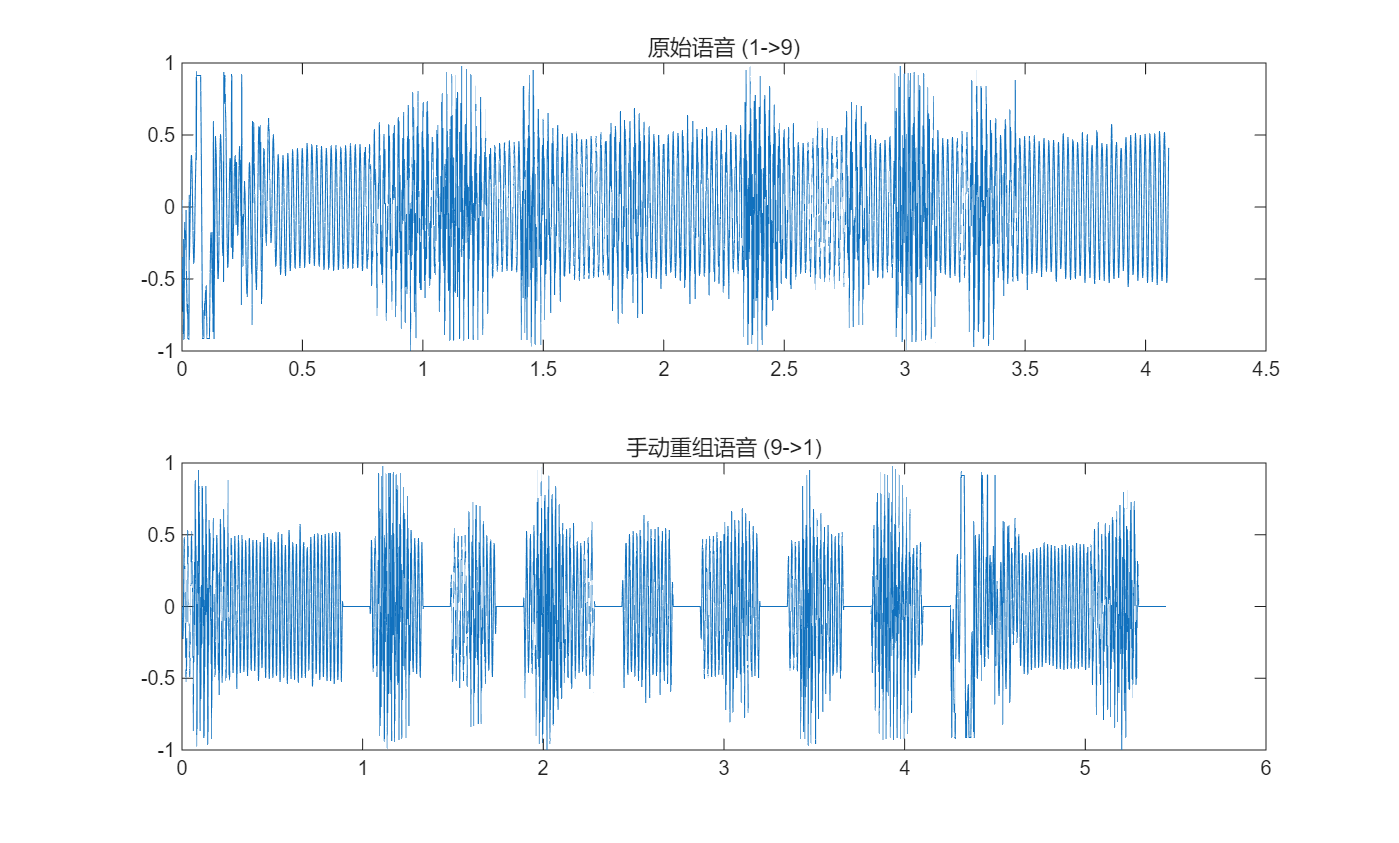
\includegraphics[width=0.9\textwidth]{./task4/untitled.png}
    % \fbox{\parbox[c][8cm][c]{14cm}{\centering [此处插入波形对比图] \\ 上图：原始录音 (1 $\to$ 9) \\ 下图：重组录音 (9 $\to$ 1) \\ 重点：展示出9个清晰的波包，顺序互为镜像}}
    \caption{连读语音的语义倒序处理结果对比}
    \label{fig:semantic_reverse}
\end{figure}

\newpage
% =========================================================
% 任务二与三：变调变速系统的算法原理与演进
% =========================================================

\section{任务二与三：音频变调变速算法设计}

\subsection{时频耦合特性}
改变音频播放速度通常会导致音调改变，这源于傅里叶变换的尺度缩放性质。若将时间轴压缩为 $1/a$，其频谱扩展 $a$ 倍。
\begin{equation}
    x(at) \leftrightarrow \frac{1}{|a|} X\left(\frac{\omega}{a}\right)
\end{equation}
这种耦合特性使得全局变换无法实现“变调不变速”或“变速不变调”。必须引入短时分析技术解决该问题。变调不变速可通过重采样配合变速不变调实现，因此本节重点讨论变速不变调算法。

\subsection{基础方案：重叠相加法 (OLA)}

\subsubsection{时域切片与重组}
重叠相加法（OLA）通过改变分析帧与合成帧的相对密度来实现时间伸缩。
如图 \ref{fig:ola_timeline} 所示：
\begin{itemize}
    \item \textbf{分析时间轴}：以固定步长 $H_a$ 截取数据。
    \item \textbf{合成时间轴}：以新步长 $H_s$ 放置数据。
\end{itemize}

\begin{figure}[H]
    \centering
    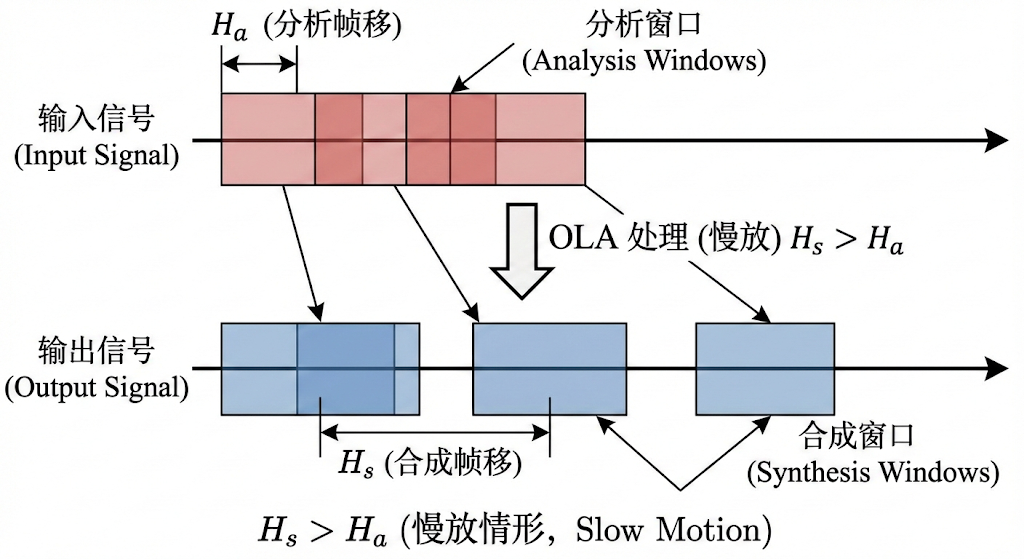
\includegraphics[width=0.8\textwidth]{./task3/ola_timeline.png}
    % \fbox{\parbox[c][7cm][c]{14cm}{\centering [此处插入 OLA 时间轴对比图] \\ 上方画原信号和紧密的 $H_a$ 窗口 \\ 下方画拉伸后的信号和稀疏的 $H_s$ 窗口 ($H_s > H_a$) \\ 用箭头标示出 $H_a$ 和 $H_s$ 的差异}}
    \caption{OLA 算法中分析帧移 $H_a$ 与合成帧移 $H_s$ 的关系示意图}
    \label{fig:ola_timeline}
\end{figure}

时间伸缩比 $\alpha = H_s / H_a$。

\subsubsection{OLA算法的相位失配问题}
OLA 虽然改变了时长，但在帧拼接处存在缺陷。
强制按照 $H_s$ 步长叠加时，前一帧尾部与后一帧头部往往存在相位差异。如图 \ref{fig:ola_mismatch} 所示，这种拼接会导致波形跳变，听觉上表现为机械噪音和颤动感，影响语音自然度。

\begin{figure}[H]
    \centering
    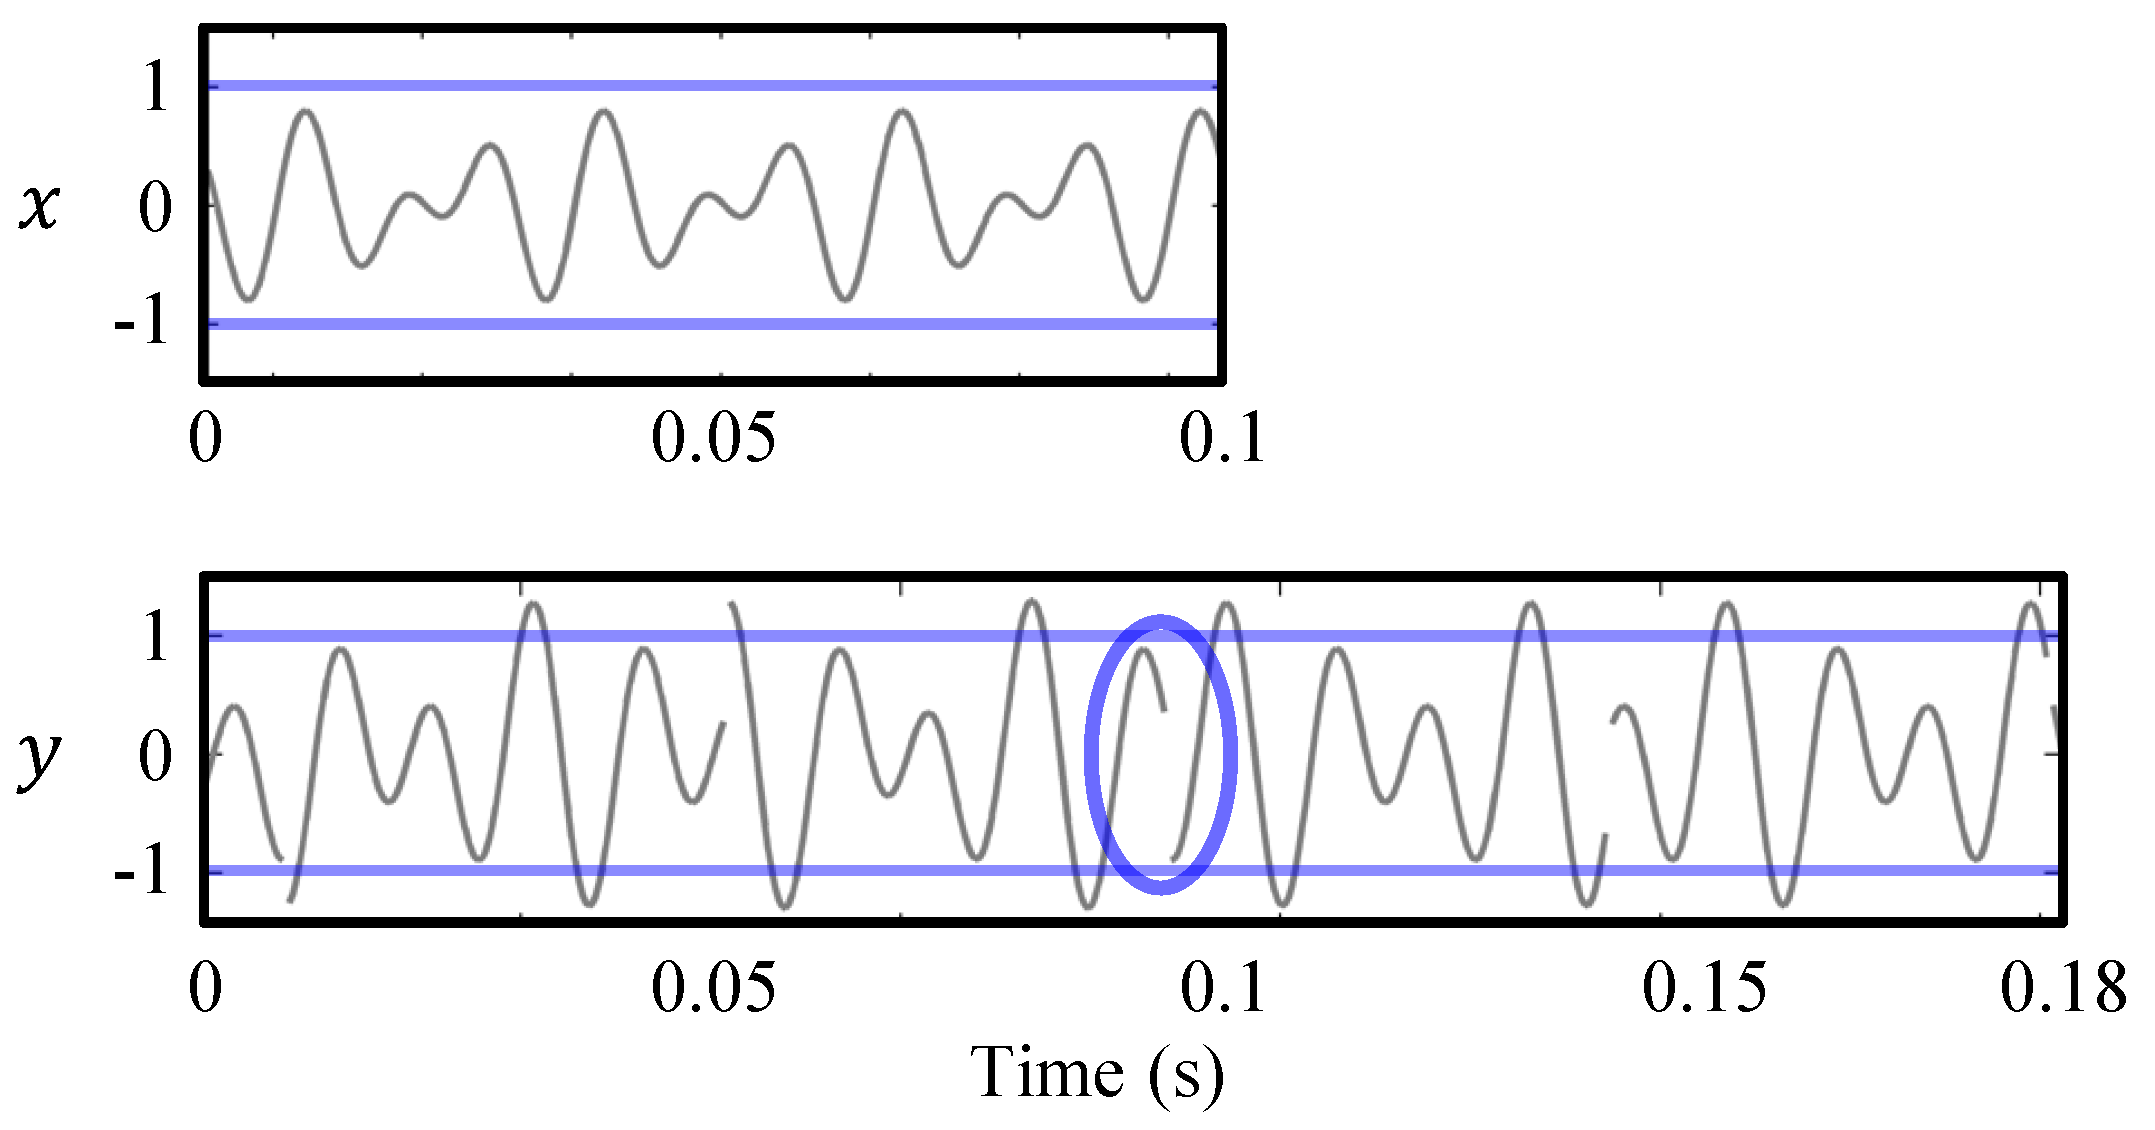
\includegraphics[width=0.8\textwidth]{./task3/ola_mismatch.png}
    % \fbox{\parbox[c][6cm][c]{12cm}{\centering [此处插入 OLA 相位失配细节图] \\ 放大展示两帧叠加区域 \\ 清晰标示出第一帧尾部和第二帧头部波形的不重合/断裂现象}}
    \caption{传统 OLA 算法导致的波形相位不连续现象}
    \label{fig:ola_mismatch}
\end{figure}

\subsection{时域改进算法：WSOLA}

\subsubsection{核心思想}

WSOLA 算法的核心是不直接截取下一帧，而是在目标位置附近寻找最自然的过渡点。

假设已合成前 $k-1$ 帧，第 $k$ 帧理想起始位置为 $L_k$。WSOLA 在 $L_k$ 附近的公差窗口内寻找一段与已合成信号尾部最相似的波形作为下一帧。

\subsubsection{实现机制}
这种“最相似”的寻找过程通过计算\textbf{归一化互相关函数（Normalized Cross-Correlation, NCC）}来实现。其数学本质等价于计算两个波形向量在高维空间中的\textbf{余弦相似度}，旨在消除信号幅度（音量）差异的影响，仅通过波形形状的几何相似性来确定最佳相位对齐点。

设 $y[n]$ 为已合成信号的尾部模板，$x[n]$ 为原信号在搜索窗口内的候选片段，归一化互相关函数 $R(\delta)$ 定义为：

\begin{equation}
    R(\delta) = \frac{\sum_{m=0}^{L-1} y[m] \cdot x[L_k + \delta + m]}{\sqrt{\sum_{m=0}^{L-1} (y[m])^2} \cdot \sqrt{\sum_{m=0}^{L-1} (x[L_k + \delta + m])^2}}
\end{equation}

其中 $L$ 为匹配窗口长度。算法步骤如下：
\begin{enumerate}
    \item \textbf{参考模板}：取已合成信号 $y$ 的末尾波形作为向量 $\vec{A}$。
    \item \textbf{滑动搜索}：在原信号 $L_k$ 附近的公差窗口 $[L_k - \Delta, L_k + \Delta]$ 内滑动截取向量 $\vec{B}(\delta)$。
    \item \textbf{寻找峰值}：计算所有 $\delta$ 对应的 $R(\delta)$，取最大值对应的偏移量 $\delta^*$：
    \begin{equation}
        \delta^* = \operatorname*{argmax}_{\delta \in [-\Delta, \Delta]} R(\delta)
    \end{equation}
\end{enumerate}

如图 \ref{fig:wsola_search_process} 所示，WSOLA 通过引入最佳偏移量 $\delta^*$，强制下一帧的起始相位与上一帧的结束相位保持“平行”（即余弦相似度最大），从而实现了平滑拼接。

\begin{figure}[H]
    \centering
    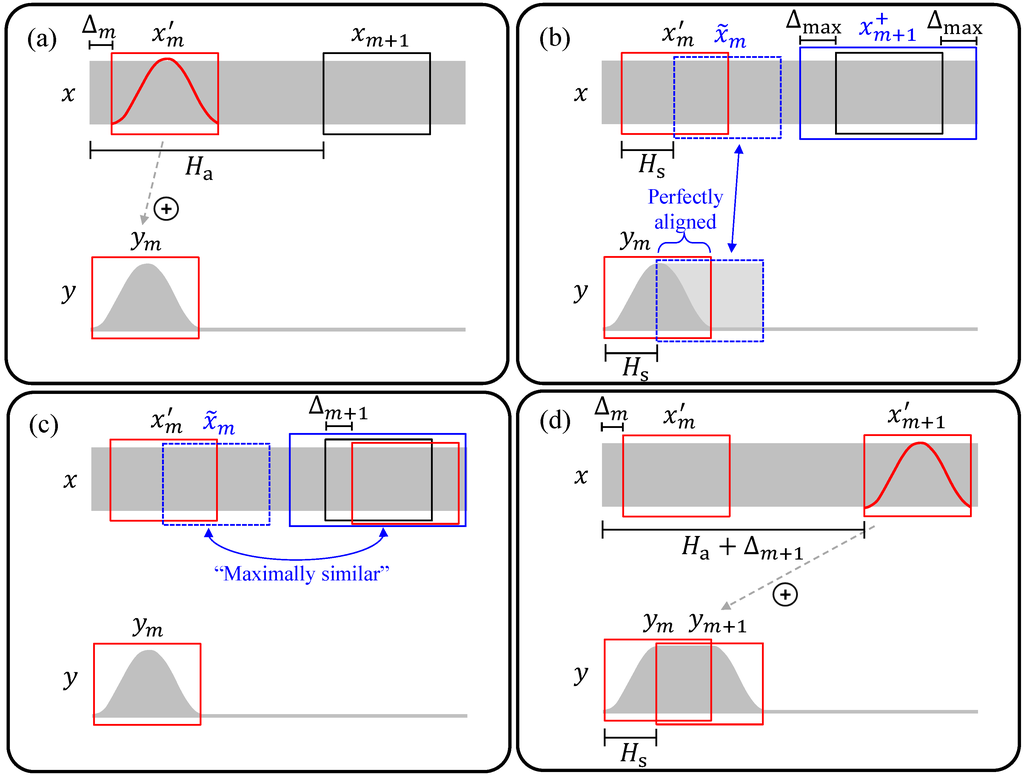
\includegraphics[width=0.95\textwidth]{./task3/wsola_mechanism.png}
    \caption{WSOLA 算法基于互相关搜索的最佳波形匹配机制}
    \label{fig:wsola_search_process}
\end{figure}

\subsection{频域改进算法：相位声码器 (Phase Vocoder)}

另一种解决相位问题的思路是利用频域方法，直接修正相位谱，即相位声码器。

\subsubsection{STFT与相位处理}
Phase Vocoder 利用 STFT 将信号分解。当改变帧跳步时，需计算各频率分量的瞬时频率，并根据新步长重新积分生成相位。

\subsubsection{相位计算}
步骤如下：
\begin{enumerate}
    \item \textbf{计算相位增量}：计算相邻两帧相位差。
    \item \textbf{计算相位偏差}：减去由固有频率产生的理论增量。
    \item \textbf{相位解卷绕}：将相位偏差映射到主值区间，估算真实瞬时频率。
    \item \textbf{相位重积分}：根据合成步长 $H_s$ 累积相位：
    \begin{equation}
        \phi_s(m) = \phi_s(m-1) + \Delta \phi_{unwrap} \cdot \frac{H_s}{H_a}
    \end{equation}
\end{enumerate}

\begin{figure}[H]
    \centering
    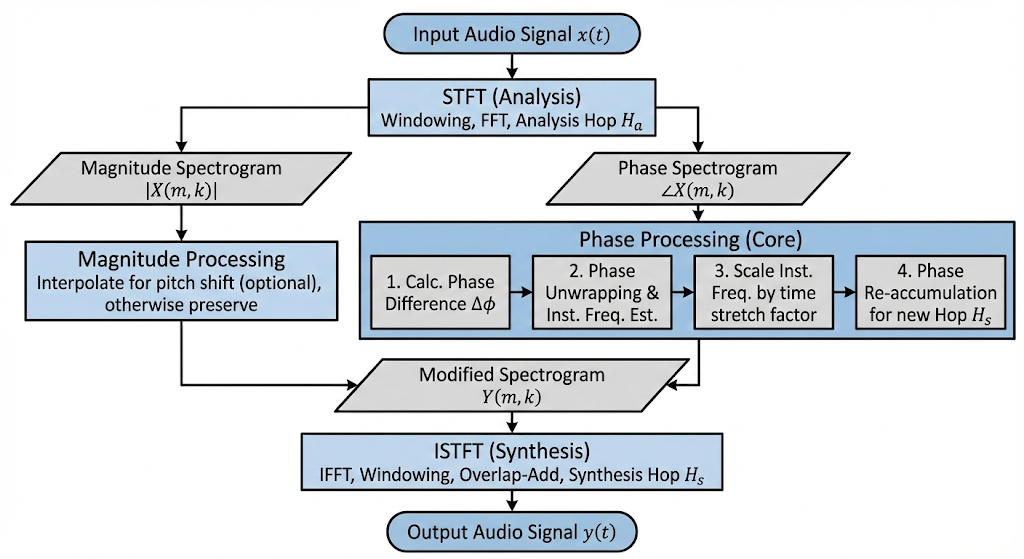
\includegraphics[width=0.95\textwidth]{./task3/pvoc_flow.png}
    \caption{Phase Vocoder 信号处理流程}
    \label{fig:pvoc_flow}
\end{figure}

\subsection{算法对比}

\begin{table}[H]
    \centering
    \caption{WSOLA 与 Phase Vocoder 算法特性对比}
    \begin{tabular}{lll}
        \toprule
        \textbf{特性} & \textbf{WSOLA (时域)} & \textbf{Phase Vocoder (频域)} \\
        \midrule
        \textbf{原理} & 波形相似性拼接 & 瞬时频率估计与相位积分 \\
        \textbf{复杂度} & 低 & 高 (需FFT/IFFT) \\
        \textbf{瞬态响应} & \textbf{较好} & 一般 (有模糊感) \\
        \textbf{相位连续性} & 依赖匹配精度 & \textbf{较好} (数学连续) \\
        \textbf{适用场景} & 语音、打击乐 & 多声部音乐 \\
        \bottomrule
    \end{tabular}
\end{table}

\subsection{实验结果与对比分析}

选取男声语音信号作为输入，分别在“变速不变调”和“变调不变速”场景下对比 WSOLA 和 Phase Vocoder (PV) 算法。

\subsubsection{场景一：变速不变调（快放）}
\textbf{1. 实验设置} \\
设定时间伸缩比 $\alpha = 0.7$（压缩至 70\%），保持音调不变。

\textbf{2. 结果分析} \\
图 \ref{fig:speed_compare} 为处理前后语谱图。
\begin{itemize}
    \item \textbf{时长控制}：两算法均成功压缩时长，且语谱图中的水平亮纹位置未偏移，说明音调未变。
    \item \textbf{细节与听感}：
    \begin{itemize}
        \item \textbf{WSOLA (图 b)}：保留了较多纹理细节。听感上清晰度较高，辅音的瞬态特征保留较好，声音较紧实。
        \item \textbf{Phase Vocoder (图 c)}：语谱图线条平滑，但听感上有一定的模糊感。由于平滑效应，瞬态冲击力有所削弱。
    \end{itemize}
\end{itemize}

\begin{figure}[H]
    \centering
    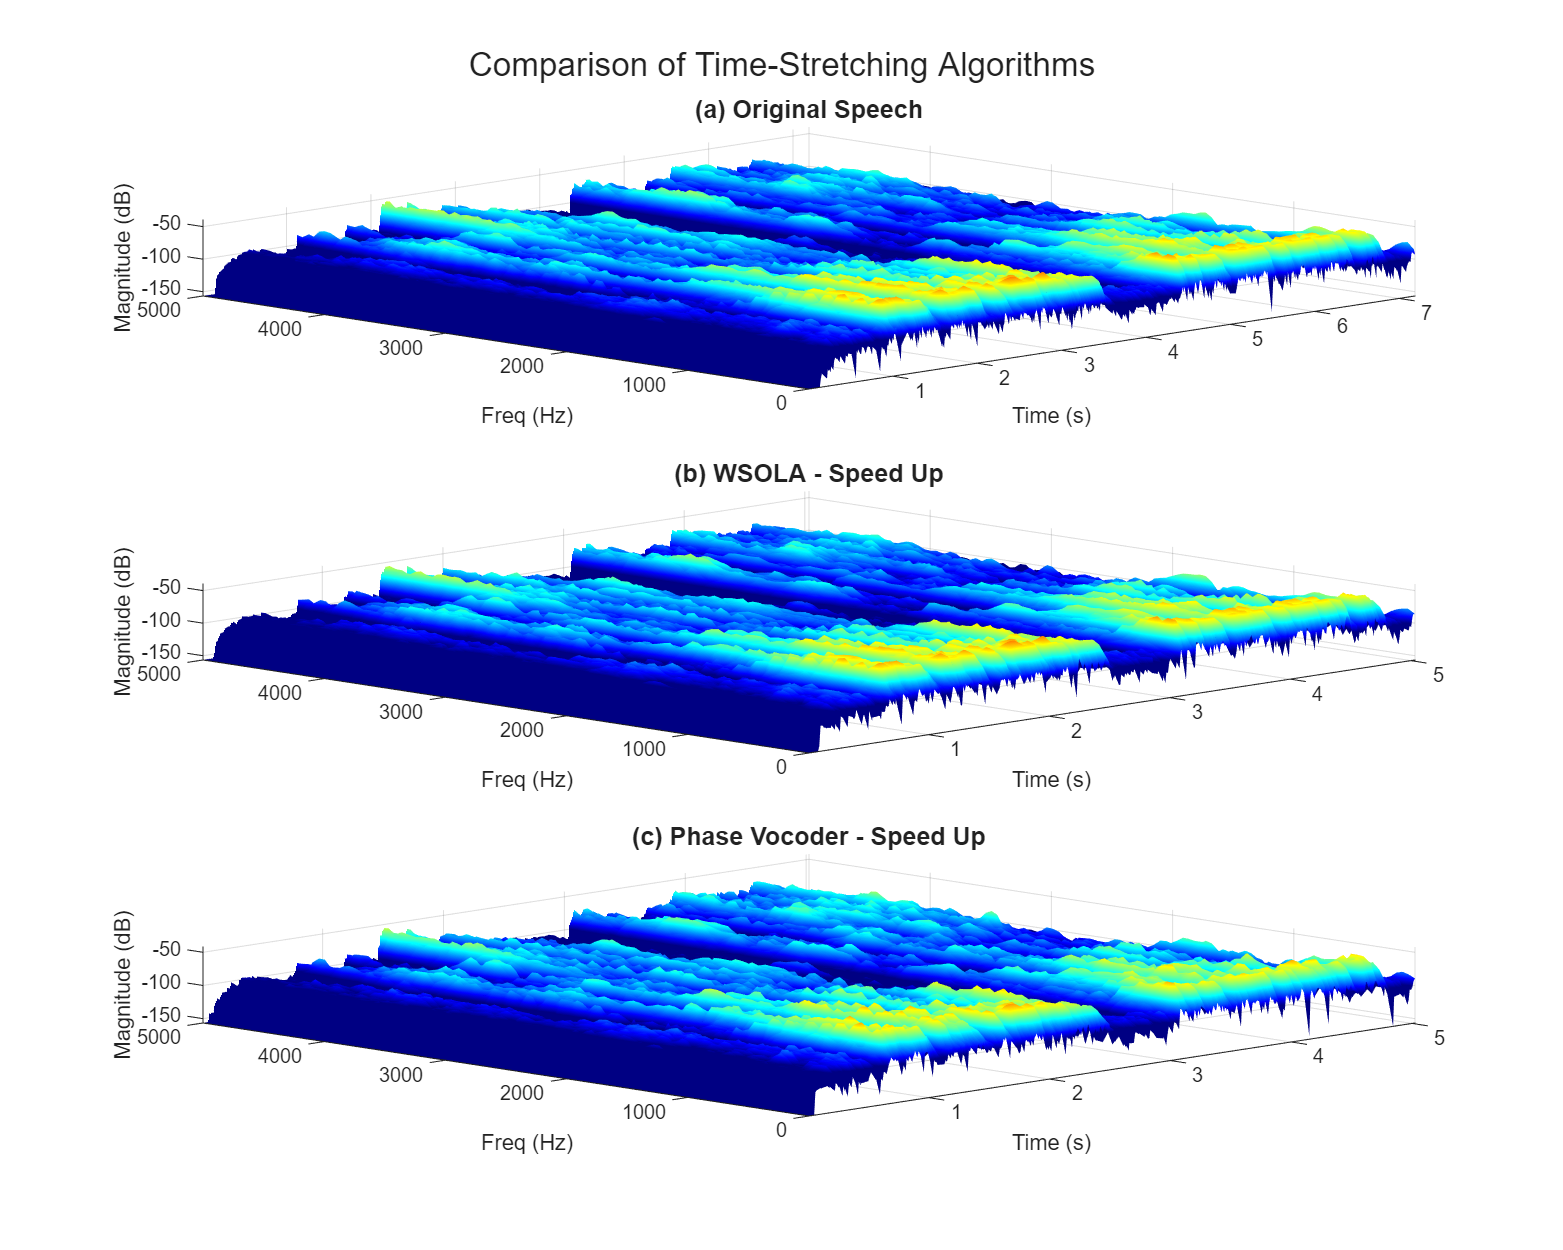
\includegraphics[width=\textwidth]{./task3/speedup.png}
    % \fbox{\parbox[c][12cm][c]{14cm}{\centering [此处插入三张语谱图 - 纵向排列] \\ (a) 原始语音 \\ (b) WSOLA 快放 0.7x \\ (c) Phase Vocoder 快放 0.7x \\ 重点：(b)纹理锐利，(c)纹理过于平滑导致模糊}}
    \caption{变速不变调（快放）实验结果对比：WSOLA vs Phase Vocoder}
    \label{fig:speed_compare}
\end{figure}

\subsubsection{场景二：变调不变速（升调）}
\textbf{1. 实验设置} \\
升高 4 个半音，时长不变。

\textbf{2. 结果分析} \\
如图 \ref{fig:pitch_compare} 所示。
\begin{itemize}
    \item \textbf{频率位移}：图 (b) 和 (c) 能量亮纹整体上移，符合升调预期。
    \item \textbf{音质分析}：
    \begin{itemize}
        \item \textbf{WSOLA (图 b)}：保留了波形内部结构，听感较自然，类似真实改变音高。
        \item \textbf{Phase Vocoder (图 c)}：存在不足。虽然水平相位连续，但破坏了频率分量间的垂直相位同步，导致听感上有一定的机械金属感和空间疏离感。
    \end{itemize}
\end{itemize}

\begin{figure}[H]
    \centering
    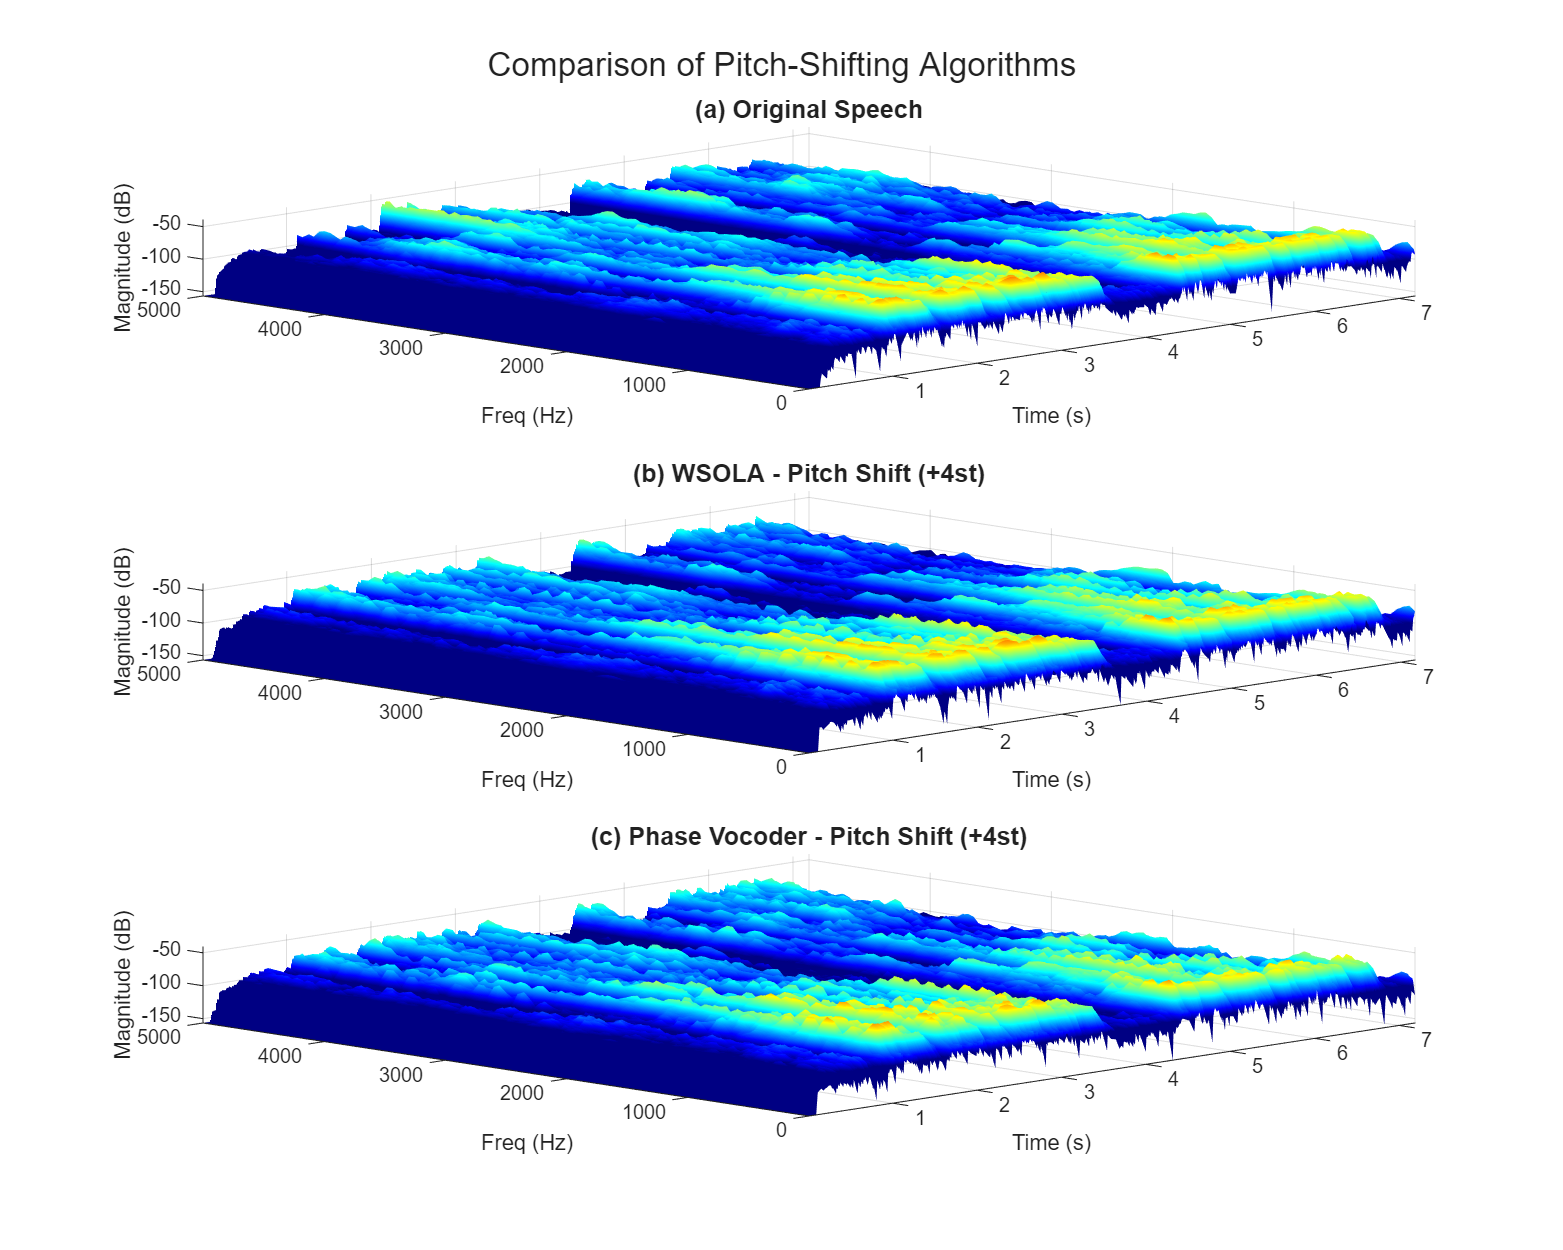
\includegraphics[width=\textwidth]{./task3/pitchup.png}
    % \fbox{\parbox[c][12cm][c]{14cm}{\centering [此处插入三张语谱图 - 纵向排列] \\ (a) 原始语音 \\ (b) WSOLA 升调 +4st \\ (c) Phase Vocoder 升调 +4st \\ 重点：(b)结构清晰，(c)虽然平滑但伴随相位失真}}
    \caption{变调不变速（升调）实验结果对比：WSOLA vs Phase Vocoder}
    \label{fig:pitch_compare}
\end{figure}

\subsubsection{小结}
对比实验表明：
\begin{enumerate}
    \item \textbf{Phase Vocoder} 虽然语谱图视觉平滑，但存在牺牲瞬态清晰度和垂直相位同步的问题，导致听感不够自然。
    \item \textbf{WSOLA} 通过复用原始波形片段，较好地维持了谐波相位关系和瞬态特征。在单声道语音处理任务中，其听感清晰度和自然度优于 Phase Vocoder。
\end{enumerate}
这说明在语音处理中，保持时域波形的完整性比单纯追求频域相位的连续性更为重要。

\newpage

% =========================================================
% 实验总结与心得
% =========================================================

\section{实验总结与心得}

本次《信号与系统》实验大作业涵盖了滤波器设计及语音变速变调算法实现。通过理论推导、MATLAB 仿真及对比分析，加深了对课程知识的理解，并锻炼了工程实践能力。

\subsection{主要结论}
\begin{enumerate}
    \item \textbf{时频耦合问题}：实验验证了傅里叶变换的尺度缩放性质。简单线性变换无法满足语音处理需求，需引入短时分析或时域拼接技术。
    \item \textbf{算法性能对比}：实验结果显示，在语音处理方面：
    \begin{itemize}
        \item \textbf{Phase Vocoder} 虽然消除了明显的断裂音，但破坏了信号在垂直方向上的相位同步，导致声音存在机械感。
        \item \textbf{WSOLA} 虽然原理简单，但通过保留原始波形片段，较好地维持了相位关系。在单声道语音处理中，其效果优于 Phase Vocoder。
    \end{itemize}
    这说明算法并非越复杂效果越好，针对具体信号特征选择合适的方法更为关键。
\end{enumerate}

\subsection{心得与体会}
\begin{itemize}
    \item \textbf{理论到实践的转化}：在设计 1800Hz 陷波器时，通过推导零极点位置并映射到 Z 平面，直观理解了系统函数与频率响应的几何关系，加深了对 Z 变换物理意义的认识。
    \item \textbf{数据分析手段}：学会了使用语谱图分析信号时频特性。通过观察能量纹理，能捕捉到时域波形难以发现的失真细节。
    % \item \textbf{调试过程体会}：编写 WSOLA 算法时曾遇到拼接噪声和数组越界问题。通过打印索引、绘制中间波形排查逻辑错误，锻炼了代码调试能力。
\end{itemize}

\subsection{不足与展望}
目前实现的算法在进行大幅度变调（如男变女）时，仅改变了基频，未调整声道共振峰，导致音色听起来像“假声”。未来可尝试引入源-滤波器模型，或基于深度学习的方法，以实现更自然的音色转换。


\begin{flushright}
    \textbf{报告人：} 郭浩然 \\
    \textbf{日期：} \today
\end{flushright}

% ... 正文结束 ...

\newpage
\appendix
\section{附录：MATLAB 核心源码}

% ==========================================
% 任务一
% ==========================================
\subsection{任务一：特定频率噪声抑制}

\subsubsection{主程序 (code1.m)}
% 注意路径：直接指向 task1 文件夹
\inputminted{matlab}{task1/code1.m}

\subsubsection{绘图脚本 A (figA.m)}
\inputminted{matlab}{task1/figA.m}

\subsubsection{绘图脚本 B (figB.m)}
\inputminted{matlab}{task1/figB.m}

% ==========================================
% 任务三
% ==========================================
\subsection{任务二、三：变速变调算法}

\subsubsection{WSOLA 算法实现 (wsola.m)}
\inputminted{matlab}{task3/wsola.m}

\subsubsection{Phase Vocoder 核心 (pv\_core.m)}
\inputminted{matlab}{task3/pv_core.m}

\subsubsection{结果绘图 (figure\_draw.m)}
\inputminted{matlab}{task3/figure_draw.m}

% ==========================================
% 任务四
% ==========================================
\subsection{任务四：语音倒放}

\subsubsection{倒放实现 (code.m)}
\inputminted{matlab}{task4/code.m}

\end{document}

\end{document}